\documentclass{article}
\usepackage[utf8]{inputenc}
\usepackage{amsmath}
\usepackage{graphicx}
\usepackage[style=authoryear, backend=biber]{biblatex} % 使用biblatex
\addbibresource{references.bib} % 确保你的.bib文件名称正确
\usepackage{graphicx}
\usepackage{booktabs} % 专业表格宏包
\usepackage{array}    % 增强表格对齐
\usepackage{tabularx} % 可选:适应文本宽度
\usepackage{placeins} % 在导言区添加
\usepackage{ragged2e}  % 文本对齐优化
\usepackage{float}

\usepackage{threeparttable} % 表格注释支持
\newcolumntype{Y}{>{\RaggedRight\arraybackslash}X} % 自适应左对齐列

\usepackage{multirow} % 合并单元格(用于处理并列排名)

\graphicspath{{images/}} % 指定图片路径

\usepackage{subcaption}  % 关键宏包必须加载
\usepackage{geometry}
\geometry{a4paper, margin=1.5cm}

% 正确定义子表格模板
\newcommand{\metricstable}[3]{%
  \begin{minipage}{0.32\textwidth}
  \centering
  \begin{tabularx}{\linewidth}{@{} >{\raggedright\arraybackslash}X r @{}}
    \toprule
    \textbf{Institution} & \textbf{#2} \\
    \midrule
    #3
    \bottomrule
  \end{tabularx}
  \end{minipage}
}


\title{Your Title Here}
\author{Your Name}
\date{\today}

\begin{document}

\maketitle

\section{Introduction}

  Modern logistics has evolved into a vital enabler of global economic integration, facilitating the seamless flow of goods across production, distribution, and consumption networks. Driven by technological innovation and sustainability imperatives, the industry is undergoing transformative shifts. Recent advancements emphasize the integration of automation and artificial intelligence, with smart warehouses and real-time tracking systems significantly enhancing operational efficiency (\cite{WOS001352081800001}). Concurrently, green logistics initiatives are reshaping traditional practices, prioritizing energy-efficient transportation and recyclable materials to align with global environmental goals (\cite{WOS:000693009900004}).

Drone technology has achieved significant breakthroughs in autonomous navigation and operational capabilities through recent advancements. Modern systems employ multi-sensor fusion architectures combining LiDAR, visual SLAM, and millimeter-wave radar to achieve centimeter-level positioning accuracy in GNSS-denied environments  (\cite{WOS:001140699200001}). The introduction of hydrogen fuel cells have significantly extended operational endurance, overcoming traditional limitations while maintaining eco-friendly profiles  (\cite{WOS:001139514900001}).

Artificial intelligence has revolutionized drone capabilities, empowering intelligent swarm coordination and real-time environmental adaptation. Vision-based navigation techniques enable dynamic route optimization and obstacle avoidance, particularly valuable for tasks like precision agriculture and infrastructure inspection  (\cite{WOS:000939165400001}). Communication breakthroughs, such as 5G-enabled edge computing, provide ultra-low latency control essential for beyond visual line of sight operations and urban air mobility networks  (\cite{WOS:001055864000001}).

Drone technology is reshaping logistics paradigms by introducing aerial solutions to longstanding terrestrial constraints. Unlike conventional delivery methods constrained by road infrastructure, drones leverage low-altitude airspace to establish direct point-to-point connections. This capability proves transformative for last-mile delivery, particularly in geographically challenging regions where traditional transport faces inefficiencies (\cite{WOS:001404731600001}).  By integrating multi-sensor navigation systems and hybrid propulsion technologies, drones enable time-sensitive pharmaceutical deliveries to remote clinics, emergency parts distribution for offshore wind farms, and precision inventory management in smart warehouses (\cite{WOS:001262605900001}). Their ability to bypass terrestrial bottlenecks complements existing logistics networks, creating layered delivery ecosystems where aerial routes dynamically adjust to real-time demand fluctuations. This shift not only addresses critical gaps in rural and urban last-mile logistics but also drives sustainable practices through energy-efficient operations, positioning drones as catalytic enablers for next-generation supply chain resilience.

In the field of drone logistics, literature reviews also play a critical role in synthesizing interdisciplinary advancements, identifying operational gaps, and guiding future research. For instance, Kim et al. (\cite{WOS:001323645000001}) employs text-mining techniques to map two decades of research in drone-assisted multimodal logistics, revealing distinct emphases in drone-truck, drone-ship, and drone-robot systems while highlighting latent topics like energy efficiency and regulatory alignment. Moshref-Javadi and Winkenbach’s framework highlights systemic gaps in multi-drone coordination and resupply dynamics, revealing a disconnect between academic focus on single-drone systems and real-world requirements for complex fleet coordination  (\cite{WOS:000693999200007}). Jazairy et al.’s systematic review bridges logistics management and technical research by evaluating drone potentials across 12 last-mile criteria, such as payload adaptability and noise reduction, while proposing stakeholder-specific solutions like privacy-preserving geofencing for regulators (\cite{WOS:001160422800001}).Jahani et al.’s  review employs text-mining to map drone applications across supply chains, identifying critical gaps in holistic integration studies. Their analysis reveals emerging priorities like sustainable logistics networks and multimodal traffic coordination, while emphasizing the need for pandemic-responsive delivery frameworks (\cite{WOS:001262605900001}).  Law et al.’s review evaluates drone applications in healthcare logistics, emphasizing their transformative potential in crisis response while identifying key barriers such as regulatory fragmentation and public trust  (\cite{WOS:000999662500001}).  

Bibliometrics, a quantitative research method that employs statistical and computational techniques to analyze publication patterns, citation networks, and knowledge evolution within academic domains, serves as a critical tool for mapping interdisciplinary advancements and identifying emerging trends. Its significance lies in synthesizing fragmented research landscapes, revealing collaborative networks, and prioritizing future directions through metrics such as co-citation analysis, keyword clustering, and temporal trend mapping (\cite{WOS:000958189000001}). Within drone technology research, several studies demonstrate the application of bibliometric approaches to map interdisciplinary knowledge domains. For instance, Fayyad et al. (\cite{WOS:001229751500001}) utilize scientometric analysis to categorize drone-based structural health monitoring (SHM) into four research clusters.  Rejeb et al. (\cite{WOS:000830895100002})) identify remote sensing, precision agriculture, and IoT as dominant themes in agricultural drone studies, while co-citation analysis reveals six research clusters. Iqbal et al.  (\cite{WOS:000914960100001})) highlight evolving priorities in drones for flood management, emphasizing computer vision and real-time detection systems.  Da Silva et al.  (\cite{WOS:001366904300001})) employ bibliometrics to reveal that UAVs are increasingly used over traditional forest inventories to efficiently assess variables like tree height, DBH, biomass, and canopy area through high-resolution sensors. While prior bibliometric reviews like "Analyzing Forklift and Drone Applications in Sustainable Logistics" (\cite{WOS:001329532200078}) provide initial insights into drone logistics, their broad scope—spanning both forklifts and drones—and exclusive focus on sustainability limit granular analysis of drone-specific logistics. In addition, this study remains confined to quantitative metrics, without in-depth review of the literature. It also relies on keyword-based search on data collection, which can be improved by manual screening of the search results. Our study addresses these gaps through a dedicated drone logistics bibliometric analysis, combining quantitative bibliometrics with qualitative analysis of domain-specific innovations. 

The primary objective of this bibliometric study is to systematically map and evaluate the intellectual landscape of drone logistics research, focusing on its evolution, thematic priorities, and collaborative networks. To address this aim, the analysis integrates performance metrics (publication trends, citation impact, leading countries/institutions, prominent journals, and dominant Web of Science categories) with science mapping techniques (keyword co-occurrence, co-authorship networks, bibliographic coupling, and citation dynamics) using data extracted from Scopus and Web of Science. Central research questions include: 


(1) Identification of seminal publications and key contributors shaping the foundation of drone logistics research.
(2) Semantic clustering of research streams and thematic evolution in the field of drone logistics.
(3) Temporal dynamics of collaboration networks and emerging frontiers in drone logistics research.

The paper is structured as follows: The methods section details the data collection protocol, including database selection, search queries, inclusion/exclusion criteria, and analytical tools. The results section presents bibliometric outputs: temporal publication trends, leading contributing countries, high-impact journals, and keyword co-occurrence clusters. The discussions section integrates these metrics with a qualitative synthesis of key literature, categorizing the field into subdomains and evaluating their interconnections, gaps, and evolution over time. The conclusions section summarizes the findings of the study, acknowledges limitations and proposes future research directions.




\section{Methods}
\subsection{Data Collection} % 二级标题
Data extraction was conducted via the Web of Science (WOS) Core Collection. The search strategy combined drone-related terms (TS=("drone*" OR "Unmanned Aerial Vehicle" OR "UAV" OR "Unmanned Aerial System" OR "UAS")) with logistics-focused queries (TS=("logistic*" OR "transport*" OR "supply chain*" OR "delivery" OR "warehouse*")) using the Boolean operator AND, executed on April 1, 2025, yielding 5,649 initial records. Manual screening of titles and abstracts excluded 3,833 publications irrelevant to drone logistics applications (e.g., agricultural monitoring, cinematography). The final dataset comprised 1,816 papers, with metadata fields (authors, institutions, keywords, citations) exported for bibliometric processing.

\section{Results}
\subsection{Publication Volume}
 The analysis of annual publication counts reveals distinct patterns in research activity within this field. From 1997 to 2017, annual outputs remained below 20 publications, with initial stagnation (1 publication in 1997, fluctuating between 2–18 until 2017). A marked acceleration began in 2018, as publications surged from 42 to 450 by 2024, corresponding to a compound annual growth rate (CAGR) of 48\% over this six-year period. Annual growth rates varied significantly, peaking at 114\% between 2019–2020 (71→152 publications), followed by gradual moderation in percentage terms. Absolute annual increments exceeded 30 publications after 2020, reaching a maximum increase of 104 publications from 2023 to 2024 (346→450). These quantitative metrics demonstrate a sustained expansion of research engagement post-2018, with publication volume increasing 10.7-fold between 2018 and 2024.

\begin{figure}[htbp]
  \centering
  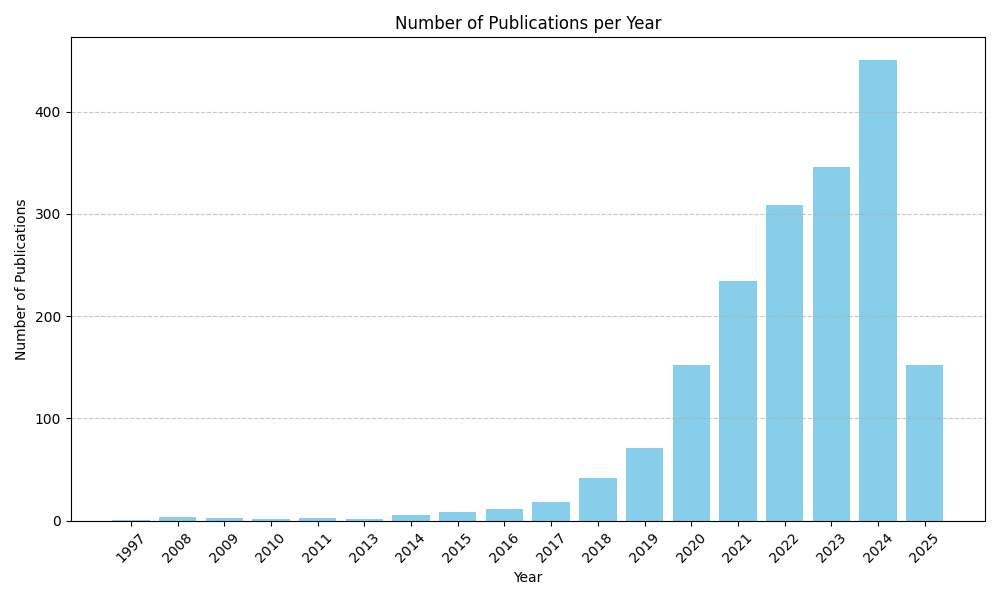
\includegraphics[width=\textwidth, keepaspectratio]{images/Figure_1}
  \caption{Number of publications per year}
  \label{fig:Figure}
\end{figure}

\subsection{Keywords}
"A systematic analysis of keyword frequencies in drone logistics literature identifies three principal categories: (1) Platform terminology with drone (347) and unmanned aerial vehicle (316) as dominant descriptors, accompanied by operational concerns like energy consumption (23) and urban air mobility (24); (2) Navigation methodologies where routing (90) and path planning (57) form the core, supported by established optimization frameworks including vehicle routing problem (27) and traveling salesman problem (24); (3) Application contexts led by logistics (80) and drone delivery (79), with last-mile delivery (50) and parcel delivery (23) as specialized sub-themes. This keyword distribution pattern shows delivery applications exhibit fewer distinct high-frequency descriptors compared to platform technologies and navigation algorithms, where drone (347), unmanned aerial vehicle (316), routing (90), and their derivative terms form a denser lexical network.

\begin{table}[htbp]
  \centering
  \caption{High-frequency Keywords in Drone Logistics Research}
  \label{tab:keyword_frequency}
  \begin{tabular}{@{} l r @{}} % 左对齐关键词,右对齐频率
    \toprule
    \textbf{Keyword} & \textbf{Frequency} \\
    \midrule
    Drone & 347 \\
    Unmanned aerial vehicle & 316 \\
    Routing & 90 \\
    Logistics & 80 \\
    Drone delivery & 79 \\
    Path planning & 57 \\
    Last-mile delivery & 50 \\
    Optimization & 43 \\
    Vehicle routing & 39 \\
    Delivery & 31 \\
    Transportation & 31 \\
    Covid-19 & 30 \\
    Vehicle routing problem & 27 \\
    Humanitarian logistics & 25 \\
    Traveling salesman problem & 24 \\
    Urban air mobility & 24 \\
    Parcel delivery & 23 \\
    Energy consumption & 23 \\
    Trajectory & 23 \\
    Task analysis & 21 \\
    \bottomrule
  \end{tabular}
\end{table}

\subsection{Authors}
Our analysis of highly cited authors in the drone logistics domain reveals Jinsoo Hwang from Sejong University as the most highly-cited scholar, with a total citation count of 1,434. Hwang’s research focuses on consumer behavior and technology adoption in drone food delivery services, with his seminal works addressing critical dimensions of service innovation (\cite{WOS:000478712400012}), risk perception (\cite{WOS:000495004400013}), and behavioral adoption (\cite{WOS:000605628800016}). Our analysis further identifies Chase C. Murray from Auburn University as the second most influential scholar in drone logistics, with a total citation count of 1,209. Murray’s research pioneers operational optimization in drone-assisted delivery systems, particularly through algorithmic innovations for truck-drone coordination, epitomized by his seminal work "The flying sidekick traveling salesman problem: Optimization of drone-assisted parcel delivery" (\cite{WOS:000353871700006}). To our knowlege, it is the first study to formalize the synchronized truck-drone routing problem as a novel variant of the vehicle routing problem (VRP). Stefan Poikonen from the University of Colorado Denver made contributions to drone logistics through his research on vehicle routing problems with drones (VRPD). His work set up theoretical frameworks for optimizing truck-drone coordination systems, introducing worst-case analyses (\cite{WOS:000400384200003}) and branch-and-bound algorithms (\cite{WOS:000468604000010}) to address operational challenges like synchronization and endurance constraints. Seokcheon Lee from Purdue University has advanced drone logistics through innovative models for truck-drone coordinated delivery systems, focusing on scalability and real-world constraints. His work "Multiple traveling salesman problem with drones: Mathematical model and heuristic approach" (\cite{WOS:000460496000002}) introduced a multi-truck-drone routing framework using mixed-integer programming and heuristics to minimize delivery times. He further addressed payload-energy dependency and No-Fly Zones (\cite{WOS:000474324300017}), integrating battery life constraints and regulatory airspace restrictions. Kevin Dorling, Jordan Heinrichs, Jordan Messier, and Sebastian Magierowski advanced drone routing by developing multi-trip VRPs that optimize energy consumption models (payload/battery weight) and enable drone reuse. Their work introduced mixed-integer programs and simulated annealing heuristics, revealing inverse exponential cost-time tradeoffs and offering tools to balance delivery efficiency and budget constraints (\cite{WOS:000391480400007}). While individual contributions remain pivotal, several highly cited scholars in drone logistics have achieved prominence through collaborative partnerships. For example, Amanda G. Chu's citation impact stems largely from co-authoring Chase C. Murray's foundational work on truck-drone routing optimization  (\cite{WOS:000353871700006}). Similarly, Jinkyung Jenny Kim’s influential studies on consumer behavior in drone food delivery emerged from collaborations with Jinsoo Hwang (\cite{WOS:000514800800001, WOS:000605628800016, WOS:000623397300001}), while Bruce Golden’s theoretical advances in vehicle routing problems with drones were co-developed with Stefan Poikonen(\cite{WOS:000400384200003, WOS:000468604000010}).

\begin{table}[htbp]
  \centering
  \caption{Top Cited Authors in Drone Logistics Research}
  \label{tab:ranked_authors}
  \begin{tabular}{@{} c l r @{}} % 三列:居中排名,左对齐作者,右对齐引用次数
    \toprule
    \textbf{Rank} & \textbf{Author} & \textbf{Citations} \\
    \midrule
    1 & Hwang, J & 1434 \\
    2 & Murray, CC & 1235 \\
    3 & Chu, AG & 920 \\
    4 & Poikonen, S & 867 \\
    5 & Lee, S & 857 \\
    6 & Kim, JJ & 812 \\
    7 & Golden, B & 784 \\
    \multirow{4}{*}{8} & Dorling, K & 766 \\ % 合并排名单元格
                        & Heinrichs, J & 766 \\
                        & Messier, GG & 766 \\
                        & Magierowski, S & 766 \\
    \bottomrule
  \end{tabular}
\end{table}

\FloatBarrier % 后续内容不会越过此屏障

\subsection{Citation analysis}
Our analysis of the most highly cited drone logistics literature begins with the top two papers—Murray et al.'s "The flying sidekick traveling salesman problem: Optimization of drone-assisted parcel delivery" (\cite{WOS:000353871700006}) and Dorling et al.'s "Vehicle Routing Problems for Drone Delivery" (\cite{WOS:000391480400007})—both previously detailed in discussions of their authors' contributions. Moving to next highly cited works: Menouar et al.'s "UAV-Enabled Intelligent Transportation Systems for the Smart City: Applications and Challenges" (\cite{WOS:000398037700003}) maps UAV applications in urban mobility, identifying key challenges like airspace regulation and cybersecurity for smart-city integration. Büyüközkan \& Gocer's "Digital Supply Chain: Literature review and a proposed framework for future research" (\cite{WOS:000432504700016}) frames drones as a pillar of digitized supply chains, emphasizing their role in agility and IoT-driven automation. Agatz et al.'s "Optimization Approaches for the Traveling Salesman Problem with Drone" (\cite{WOS:000442591800013}) formalizes the TSP-D model for truck-drone coordinated delivery, proposing route-first-cluster-second heuristics to minimize last-mile costs. Their work demonstrate substantial savings over truck-only systems. Ha et al.'s "On the min-cost Traveling Salesman Problem with Drone" (\cite{WOS:000442591800013}) introduces a cost-centric TSP-D variant, proposing a Greedy Randomized Adaptive Search Procedure (GRASP) heuristics to minimize operational expenses, including vehicle wait times. Zeng et al.'s "From high-touch to high-tech: COVID-19 drives robotics adoption" (\cite{WOS:000534121800001}) documents how the pandemic accelerated drone deployment for contactless logistics, particularly in healthcare and tourism. The study forecasts a permanent shift toward hybrid human-robot workflows, despite ethical debates on job displacement. Wang et al.'s "The vehicle routing problem with drones: several worst-case results" (\cite{WOS:000400384200003}) establishes theoretical bounds for truck-drone coordinated efficiency, proving that drone speed and fleet size dictate maximum time savings. Stolaroff et al.'s "Energy use and life cycle greenhouse gas emissions of drones for commercial package delivery" (\cite{WOS:000424872000001}) employs lifecycle assessment (LCA) for drone-based delivery, revealing that small drones exhibit lower per-package energy consumption than ground vehicles for short-haul trips. However, the study cautions that expanded warehouse networks and longer flight paths can offset these gains. Their findings conclude that, with optimized infrastructure and drone size, drone delivery systems hold potential to reduce greenhouse gas emissions compared to conventional logistics.Wang \& Sheu's "Vehicle routing problem with drones" (\cite{WOS:000465060600016}) introduces a mixed-integer programming model for the vehicle routing problem with drones (VRPD), extending classical capacitated VRP to accommodate dynamic drone redeployment across trucks. Their branch-and-price algorithm optimizes integrated truck-drone routing under flying range and payload constraints, with extensive experiments on practically generated instances demonstrating the algorithm’s robust computational performance.


\begin{table}[htbp]
  \centering
  \caption{Top Cited Articles in Drone Logistics Research (2010-2023)}
  \label{tab:top_articles}
  \begin{tabularx}{\textwidth}{@{} >{\centering\arraybackslash}p{1.5cm} X r @{}}
    \toprule
    \textbf{Rank} & \textbf{Article Title} & \textbf{Citations} \\
    \midrule
    1 & The flying sidekick traveling salesman problem: Optimization of drone-assisted parcel delivery & 920 \\
    2 & Vehicle Routing Problems for Drone Delivery & 766 \\
    3 & UAV-Enabled Intelligent Transportation Systems for the Smart City: Applications and Challenges & 609 \\
    4 & Digital Supply Chain: Literature review and a proposed framework for future research & 579 \\
    5 & Optimization Approaches for the Traveling Salesman Problem with Drone & 523 \\
    6 & On the min-cost Traveling Salesman Problem with Drone & 375 \\
    7 & From high-touch to high-tech: COVID-19 drives robotics adoption & 336 \\
    8 & The vehicle routing problem with drones: several worst-case results & 325 \\
    9 & Energy use and life cycle greenhouse gas emissions of drones for commercial package delivery & 316 \\
    10 & Vehicle routing problem with drones & 311 \\
    \bottomrule
  \end{tabularx}
\end{table}

\FloatBarrier % 后续内容不会越过此屏障

\subsection{Countries}
The analysis of national contributions to drone logistics research reveals a clear hierarchy in drone logistics research contributions across countries, measured by publication volume, citation impact, and H-index. The United States leads in citation impact (13,548 citations) and H-index (56), despite ranking second in publication count (383 studies), underscoring its dominant role in high-impact research. China ranks first in publication volume (528 studies) but second in citations (8,437) and H-index (45), reflecting a large-scale output with relatively lower per-study impact compared to the U.S. South Korea holds third place across all metrics (138 publications, 4,493 citations, H-index 36), demonstrating balanced productivity and impact.

European nations like Germany (82 studies) and Italy (83 studies) achieve identical H-indices (27), demonstrating comparable scholarly influence at a moderate output level. Canada (75 publications, H-index 23) and Australia (72 publications, H-index 24) exhibit efficient research ecosystems with mid-tier citation traction (2,898 and 1,915 citations, respectively). India, while emerging as an active contributor (109 publications), show lower H-indices (21), indicating room for greater global impact.


\begin{table}[htbp]
  \centering
  \caption{National Research Output Metrics in Drone Logistics}
  \label{tab:research_metrics}
  \begin{tabularx}{0.9\textwidth}{@{} >{\RaggedRight}p{3cm} r r r @{}}
    \toprule
    \textbf{Country} & \textbf{Publications} & \textbf{Total Citations} & \textbf{H-index} \\
    \midrule
    USA              & 383  & 13548 & 56 \\
    Peoples R China  & 528  & 8437  & 45 \\
    South Korea      & 138  & 4493  & 36 \\
    Germany          & 82   & 2604  & 27 \\
    Italy            & 83   & 2023  & 27 \\
    England          & 110  & 1977  & 26 \\
    Australia        & 72   & 1915  & 24 \\
    Canada           & 75   & 2898  & 23 \\
    India            & 109  & 1582  & 21 \\
    Spain            & 52   & 1388  & 19 \\
    \bottomrule
  \end{tabularx}
\end{table}

\subsection{Institutions}
In this section, we turn to analyzing high-impact institutions in drone logistics research. Sejong University emerges as a leading institution with 1,712 total citations and an H-index of 19, driven by interdisciplinary collaborations. While most of its top-cited works focus on consumer behavior and technology adoption in drone food delivery (e.g., perceived innovativeness (\cite{WOS:000478712400012}), risk perception (\cite{WOS:000495004400013}), and COVID-19 impacts (\cite{WOS:000605628800016}))—led by Jinsoo Hwang’s aforementioned behavioral science studies—its most cited paper, "Routing in Flying Ad Hoc Networks: A Comprehensive Survey" (218 citations), represents a distinct technical domain.This survey systematically categorizes routing protocols for Flying Ad Hoc Networks (FANETs), analyzing their strengths/weaknesses against challenges like high mobility and topology instability. It evaluates protocols using mobility models and proposes a taxonomy to guide future FANET communication design (\cite{WOS:000538038400010}). The institution’s research portfolio underscores a balanced emphasis on technical and socioeconomic research, positioning it as a hub for drone logistics innovation. Auburn University holds a notable position in drone logistics research with 1,062 total citations, though its influence is overwhelmingly driven by a single landmark study: "The flying sidekick traveling salesman problem" (920 citations) (\cite{WOS:000353871700006}). Purdue University's research in drone logistics spans optimization frameworks—mathematical models like insertion heuristics that handle large-scale routing across hundreds of nodes (\cite{WOS:000460496000002})—and real-world constraint modeling, which integrates operational hurdles such as battery limits (\cite{WOS:000532795300023}), No-Fly Zones (\cite{WOS:000474324300017}), and multi-trip payload fluctuations (\cite{WOS:000523602300006}). University of Maryland has 947 total citations. Its foundational work, "The vehicle routing problem with drones: several worst-case results" (\cite{WOS:000400384200003})  (325 citations), quantified the maximum time savings achievable via drones under varying speed ratios and fleet sizes. A follow-up study  (229 citations) by the same institution expanded the previous study by linking it to Amdahl’s Law, emphasizing how drones enhance efficiency via parallel task execution (\cite{WOS:000404719400004}). York University (Canada) and University of Calgary's influence in drone logistics are heavily anchored by a single landmark study: "Vehicle Routing Problems for Drone Delivery" (\cite{WOS:000391480400007}). Authored by Dorling et al., this work established energy-aware multitrip routing models, integrating linear payload-battery energy consumption into MILP formulations and simulated annealing heuristics. The University of Florida's impact in drone logistics is dominated by "UAV-Enabled Intelligent Transportation Systems for the Smart City: Applications and Challenges" (\cite{WOS:000398037700003}) (609 citations, ~74\% of total citations). This study maps UAV applications and key challenges for smart-city intelligent transportation systems. State University of New York has advanced drone logistics with 798 citations, focusing on multi-drone coordinated delivery (\cite{WOS:000509790500020}) and barrier analysis (\cite{WOS:000547773000001}).

The interplay between publication volume, H-index, and total citations reveals distinct institutional research profiles in drone logistics. Sejong University exemplifies balanced excellence, ranking 4th in output (27 papers) but 1st in both H-index (19) and total citations (1,712), underscoring its dual strength in behavioral studies (\cite{WOS:000478712400012}) and technical innovations (\cite{WOS:000538038400010}). In contrast, Hong Kong Polytechnic University leads in sheer output (42 papers) but trails in H-index (14) and total citations (absent from the top 10), reflecting a high-volume yet moderately cited portfolio. Chinese institutions like Nanjing University of Aeronautics \& Astronautics (2nd in output, 33 papers) and Beihang University (3rd, 28 papers) prioritize quantity but lack representation in H-index and citation rankings. Nanyang Technological University (6th in output, 22 papers; 3rd in H-index, 13) and University of New South Wales Sydney (3rd in H-index, 13) achieve higher per-paper impact through optimization frameworks (\cite{WOS:000501349900060}) and collaborative delivery models (\cite{WOS:000467564700204}). Tsinghua University (8th in output, 20 papers; 8th in H-index, 10), Purdue University (9th in output, 19 papers; 8th in H-index, 10) and the University of Maryland (9th in output, 19 papers; 8th in H-index, 10) demonstrate moderate yet consistent influence across output and impact metrics.



\begin{table}[htbp]
  \centering
  \caption{Top 10 Institutions by Total Citations}
  \label{tab:citations}
  \begin{tabularx}{0.9\textwidth}{@{} >{\raggedright}X r @{}}
    \toprule
    Institution & Total Citations \\
    \midrule
    Sejong University & 1712 \\
    Auburn University & 1062 \\
    Purdue University & 1041 \\
    University System of Maryland & 947 \\
    University of Maryland & 883 \\
    York University - Canada & 863 \\
    State University System of Florida & 821 \\
    University of Calgary & 807 \\
    State University of New York (SUNY) System & 798 \\
    Erasmus University Rotterdam & 763 \\
    \bottomrule
  \end{tabularx}
\end{table}

%% 表2:论文数量排名
\begin{table}[htbp]
  \centering
  \caption{Top 10 Institutions by Publications} 
  \label{tab:publications}
  \begin{tabularx}{0.9\textwidth}{@{} >{\raggedright}X r @{}}
    \toprule
    Institution & Publications \\
    \midrule
    Hong Kong Polytechnic University & 42 \\
    Nanjing University of Aeronautics \& Astronautics & 33 \\
    Beihang University & 28 \\
    Sejong University & 27 \\
    National University of Defense Technology - China & 26 \\
    Nanyang Technological University & 22 \\
    Chinese Academy of Sciences & 21 \\
    Tsinghua University & 20 \\
    Purdue University & 19 \\
    University System of Maryland & 19 \\
    \bottomrule
  \end{tabularx}
\end{table}

%% 表3:H指数排名 
\begin{table}[htbp]
  \centering
  \caption{Top 10 Institutions by H-index}
  \label{tab:hindex}
  \begin{tabularx}{0.9\textwidth}{@{} >{\raggedright}X r @{}}
    \toprule
    Institution & H-index \\
    \midrule
    Sejong University & 19 \\
    Hong Kong Polytechnic University & 14 \\
    University of New South Wales Sydney & 13 \\
    Nanyang Technological University & 13 \\
    National University of Defense Technology - China & 12 \\
    Kyung Hee University & 11 \\
    Northwestern Polytechnical University & 11 \\
    Purdue University & 10 \\
    University System of Maryland & 10 \\
    University of Missouri System & 10 \\
    \bottomrule
  \end{tabularx}
\end{table}

\subsection{Sources}
The distribution of publications and citation impact across journals reveals distinct patterns in drone logistics research. Drones leads in publication volume (98 papers) but has the lowest average citations (7.34) among top-output journals. Subsequent examination of highly cited articles in Drones suggests a focus on rapid dissemination of applied or technical studies (\cite{WOS:000682822500001, WOS:000682822500021}). Sustainability (57 papers, 16.88 avg. citations) ranks second in publication volume, reflecting its role in hosting interdisciplinary studies on drone logistics' environmental and societal impacts (\cite{WOS:000531558100214, WOS:000428567100315}). IEEE Transactions on Intelligent Transportation Systems (57 papers, 28.40 avg. citations) matches Sustainability in output but achieves higher citations, indicative of its focus on routing innovations (\cite{WOS:000658360600026}) and UAV integration into adaptive traffic systems (\cite{WOS:000684003100038}). Transportation Research Part C: Emerging Technologies (53 papers) achieves the highest average citations (79.15) in this category, reflecting its prominence in publishing high-impact applied optimization studies (\cite{WOS:000353871700006, WOS:000425566000035}). IEEE Access (46 papers, 16.00 avg. citations) and Applied Sciences-Basel (38 papers, 7.50 avg. citations) prioritize rapid dissemination of applied research, with IEEE Access showing marginally higher citation influence due to its engineering-focused scope. Transportation Research Part E: Logistics and Transportation Review (36 papers, 34.31 avg. citations) publishes strategic analyses of drone logistics' cost-efficiency and supply chain integration (\cite{WOS:000488423300001}). European Journal of Operational Research (33 papers, 29.73 avg. citations) and Computers \& Industrial Engineering (31 papers, 29.55 avg. citations) demonstrate balanced output and citations, focusing on operational research (\cite{WOS:000742554100008}) and computational methods for UAV routing (\cite{WOS:000460496000002}). Drone logistics research exhibits a dichotomy between high-output, application-focused journals (e.g., Drones with 98 papers) and lower-output, high-impact journals (e.g., Transportation Research Part C with 79.15 avg. citations).


\begin{table}[htbp]
  \centering
  \caption{Top Journals in Drone Logistics Research (2018-2023)}
  \label{tab:journals}
  \begin{tabularx}{0.9\textwidth}{@{} >{\raggedright}X r r r @{}}
    \toprule
    \textbf{Journal} & \textbf{Pubs.} & \textbf{Total Cites} & \textbf{Cites/Paper} \\
    \midrule
    Drones & 98 & 719 & 7.34 \\
    Sustainability & 57 & 962 & 16.88 \\
    IEEE Transactions on Intelligent Transportation Systems & 57 & 1619 & 28.40 \\
    Transportation Research Part C: Emerging Technologies & 53 & 4195 & 79.15 \\
    IEEE Access & 46 & 736 & 16.00 \\
    Applied Sciences-Basel & 38 & 285 & 7.50 \\
    Transportation Research Part E: Logistics and Transportation Review & 36 & 1235 & 34.31 \\
    European Journal of Operational Research & 33 & 981 & 29.73 \\
    Computers \& Industrial Engineering & 31 & 916 & 29.55 \\
    Sensors & 30 & 533 & 17.77 \\
    \bottomrule
  \end{tabularx}
  
  \vspace{0.5em}
  \raggedright\footnotesize
\end{table}

\FloatBarrier

\subsection{Discipline}
The disciplinary focus of drone logistics research has expanded significantly post-2020, reflecting evolving technological and operational priorities. Engineering, Electrical \& Electronic remains dominant (63 pre-2020 → 299 post-2020), driven by advancements in UAV hardware, energy efficiency, and IoT integration. Transportation Science \& Technology (51 → 265) and Operations Research \& Management Science (56 → 255) show accelerated growth, emphasizing route optimization and hybrid truck-drone coordinated systems. Emerging disciplines post-2020 include Management (127) and Remote Sensing (103), highlighting a shift toward strategic logistics governance and geospatial applications. The rise of Computer Science, Artificial Intelligence (26 → 108) and Remote Sensing underscores the field’s pivot toward data-driven decision-making, such as AI-enhanced routing and dynamic fleet coordination (\cite{WOS:000742554100008}). This evolution reflects drone logistics' maturation from technical feasibility (pre-2020) to multidisciplinary scalability (post-2020), bridging engineering innovations with managerial and computational advancements.

\begin{table}[H]
  \centering
  \caption{Evolution of High-Frequency Disciplines in Drone Logistics Research}
  \label{tab:discipline_evolution}
  
  \begin{minipage}[t]{0.48\textwidth}
  \centering
  \begin{tabularx}{\linewidth}{@{} >{\raggedright}X r @{}}
    \toprule
    \multicolumn{2}{c}{\textbf{Pre-2021 (2000-2020)}} \\
    \midrule
    \textbf{Discipline} & \textbf{Frequency} \\
    \midrule
    Engineering, Electrical \& Electronic & 63 \\
    Operations Research \& Management Science & 56 \\
    Transportation Science \& Technology & 51 \\
    Telecommunications & 44 \\
    Computer Science, Information Systems & 40 \\
    Transportation & 36 \\
    Robotics & 27 \\
    Computer Science, Artificial Intelligence & 26 \\
    Computer Science, Interdisciplinary Applications & 17 \\
    Engineering, Civil & 17 \\
    \bottomrule
  \end{tabularx}
  \end{minipage}
  \hfill
  \begin{minipage}[t]{0.48\textwidth}
  \centering
  \begin{tabularx}{\linewidth}{@{} >{\raggedright}X r @{}}
    \toprule
    \multicolumn{2}{c}{\textbf{Post-2021 (2021-2023)}} \\
    \midrule
    \textbf{Discipline} & \textbf{Frequency} \\
    \midrule
    Engineering, Electrical \& Electronic & 299 \\
    Transportation Science \& Technology & 265 \\
    Operations Research \& Management Science & 255 \\
    Telecommunications & 164 \\
    Computer Science, Information Systems & 150 \\
    Transportation & 142 \\
    Management & 127 \\
    Engineering, Civil & 126 \\
    Computer Science, Artificial Intelligence & 108 \\
    Remote Sensing & 103 \\
    \bottomrule
  \end{tabularx}
  \end{minipage}

  \vspace{0.5em}
  \raggedright\footnotesize
\end{table}

\FloatBarrier

\section{Discussion}
This section discusses the results

\section{Conclusion}
This is the conclusion section

\printbibliography



\end{document}